\documentclass[oneside]{book}
\usepackage{listings}
\usepackage{caption}
\usepackage{subcaption}
\usepackage[all]{xy}
\usepackage{imakeidx}
\makeindex
\usepackage{graphicx}
\usepackage[export]{adjustbox}
\usepackage[spanish]{babel}
\title{Apunte ICPC}

\begin{document}

\lstloadlanguages{C++}
\lstnewenvironment{codigo}
  {
    \lstset{
        language=C++,
        numbers=left,
        stepnumber=1,
        basicstyle=\footnotesize\ttfamily}
  }
  {
  }

\lstset{
        language=C++,
        numbers=left,
        stepnumber=1,
        tabsize=2,
        breaklines=true,
        basicstyle=\footnotesize\ttfamily}
  
	\maketitle	
	\tableofcontents

	\frontmatter
	\chapter{Notas previas}
	\section{Abreviaciones utilizadas}
	\lstinputlisting{Misc/Abreviaciones.cpp}
	\mainmatter
	\chapter{Estructuras de datos}
	\section{Fenwick Tree}
	\textbf{Nota:} Ambas implementaciones tienen rangos entre 1 a n. \index{Fenwick Tree}
	\subsection{Actualizaciones por rango, consultas puntales }
	\lstinputlisting{Estructuras/FTaRcP.cpp}
	\pagebreak
	\subsection{Actualizaciones puntuales, consultas por rango}
	La consulta $query(a,b)$ corresponde a la sumatoria de los elementos entre los \'indices $a$ y $b$. \index{RSQ}
	\lstinputlisting{Estructuras/FTaPcR.cpp}
	
	\section{Union-Find}
	Utilizada para trabajar conjuntos disjuntos. Sirve para encontrar componentes conexas en grafos no dirigidos. \index{Componentes conexas} \index{Conjuntos disjuntos} \index{Particiones}
	\lstinputlisting{Estructuras/UnionFind.cpp}
	\section{Segment Tree}
		\subsection{Iterativo}
			\lstinputlisting{Estructuras/SegTree.cpp}
		\subsection{Lazy}
			\lstinputlisting{Estructuras/SegTreeLazy.cpp}
		\subsection{Pair}
			\lstinputlisting{Estructuras/SegmentTreePair.cpp}
			
			
	\section{Wavelet Tree}
		\lstinputlisting{Estructuras/wavelet.cpp}
		
			

	
	\chapter{Grafos}
	\section{DFS}
	\lstinputlisting{Grafos/dfs.cpp}
	\section{Brexit}
	\lstinputlisting{Grafos/brexit.cpp}
	\section{Kruskal}
	\lstinputlisting{Grafos/kruskal.cpp}
	\section{Single source shortest path}
	\section{Edmond Blonsson}
	\lstinputlisting{Grafos/EdmonBlonsson.cpp}
	\section{Flood Fill}
	\lstinputlisting{Grafos/FloodFill.cpp}
	\section{Dijkstra}
	Utilizamos la representacion vvii con pares (vecino,peso)
	\begin{codigo}
	asd
	\end{codigo}
	\chapter{Matem\'atica}
	\section{Pascal}
	\lstinputlisting{Math/pascal.cpp}
	\section{Criba}
	\lstinputlisting{Math/prime_sieve.cpp}
	
	\chapter{Geometria}
	\section{Intersection}
	\lstinputlisting{Geometria/UnionFind&&Segment.cpp}
	\section{Rectangle union}
	\lstinputlisting{Geometria/rectangleunion.cpp}
	\section{Closest pair}
	\lstinputlisting{Geometria/closestpair.cpp}
	\section{Radial sweep example}
	\lstinputlisting{Geometria/hideandseek.cpp}
	\section{Line sweep example}
	\lstinputlisting{Geometria/fence.cpp}
	\chapter{Flujo}
	\section{Problemas de asignaci\'on}
	\subsection{Bipartite matching}
	\index{Bipartite matching}
	Tenemos dos conjuntos $A$ y $B$, donde cada elemento de $A$ es compatible con ciertos elementos de $B$. Adem\'as, tenemos la condici\'on de que podemos asociar cada elemento de $A$ con a lo m\'as un solo elemento de $B$. Bipartite matching nos permite saber la cantidad m\'axima de asociaciones posibles.
\begin{figure}[h]
\centering
\begin{subfigure}{.5\textwidth}
\begin{displaymath}
\xymatrix@R-1pc{
&&&*+[o][F-]{B_1} \ar[dddrr] \\
&&*+[o][F-]{A_1} \ar[ur] \ar[dr]
&*+[o][F-]{B_2} \ar[ddrr] \\
&&*+[o][F-]{A_2} \ar[r] \ar[dddr] \ar[ur]
&*+[o][F-]{B_3} \ar[drr] \\
*+[o][F-]{S} \ar[rruu] \ar[rru] \ar[rr] \ar[rrd] \ar[rrdd]
&&*+[o][F-]{A_3} \ar[ur]
&*+[o][F-]{B_4} \ar[rr]
&&*+[o][F-]{T} \\
&&*+[o][F-]{A_4} \ar[ddr]
&*+[o][F-]{B_5} \ar[urr] \\
&&*+[o][F-]{A_5} \ar[r] \ar[uur]
&*+[o][F-]{B_6} \ar[uurr] \\
&&&*+[o][F-]{B_7} \ar[uuurr]
}
\end{displaymath}
\caption*{Modelamiento utilizado. Todas las aristas llevan 1 de flujo.}
\end{subfigure}

\end{figure}

\section{Dinic}
	\lstinputlisting{Flujo/Dinic.cpp}
	\chapter{Programaci\'on din\'amica}
	\section{0/1 Knapsack}
	\lstinputlisting{DP/01knap.cpp}
	\section{Bitonic Sequence}
	\lstinputlisting{DP/BitonicSequence.cpp}
	\section{Box Stacking}
	\lstinputlisting{DP/BoxStacking.java}
	\section{Break multiple words with no space into space}
	\lstinputlisting{DP/break.java}
	\section{Burst Balloon}
	\lstinputlisting{DP/BurstBallon.java}
	\section{Catalan}
	\lstinputlisting{DP/Catalan.cpp}
	\section{Coin changing}
	\lstinputlisting{DP/CoinChanging.cpp}
	\section{Cutting sticks}
	\lstinputlisting{DP/CuttingStick.cpp}
	\section{Distinct subsequence}
	\lstinputlisting{DP/DistinctSubsequence.java}
	\section{Divide and conquer}
	\lstinputlisting{DP/DivideAndConquer.cpp}
	\section{Edit Distance}
	\lstinputlisting{DP/EditDistance.java}
	\section{Sum 2D Rectangle}
	\lstinputlisting{DP/Sum2DRectangle.java}
	\section{Sum Dice}
	\lstinputlisting{DP/SumDice.java}
	
	
	
	\chapter{Contenido adicional}
	\section{Fast input}
	\lstinputlisting{Misc/fastio.cpp}
	\section{Usar en caso de emergencia}
	\begin{figure}[h]
		\centering
		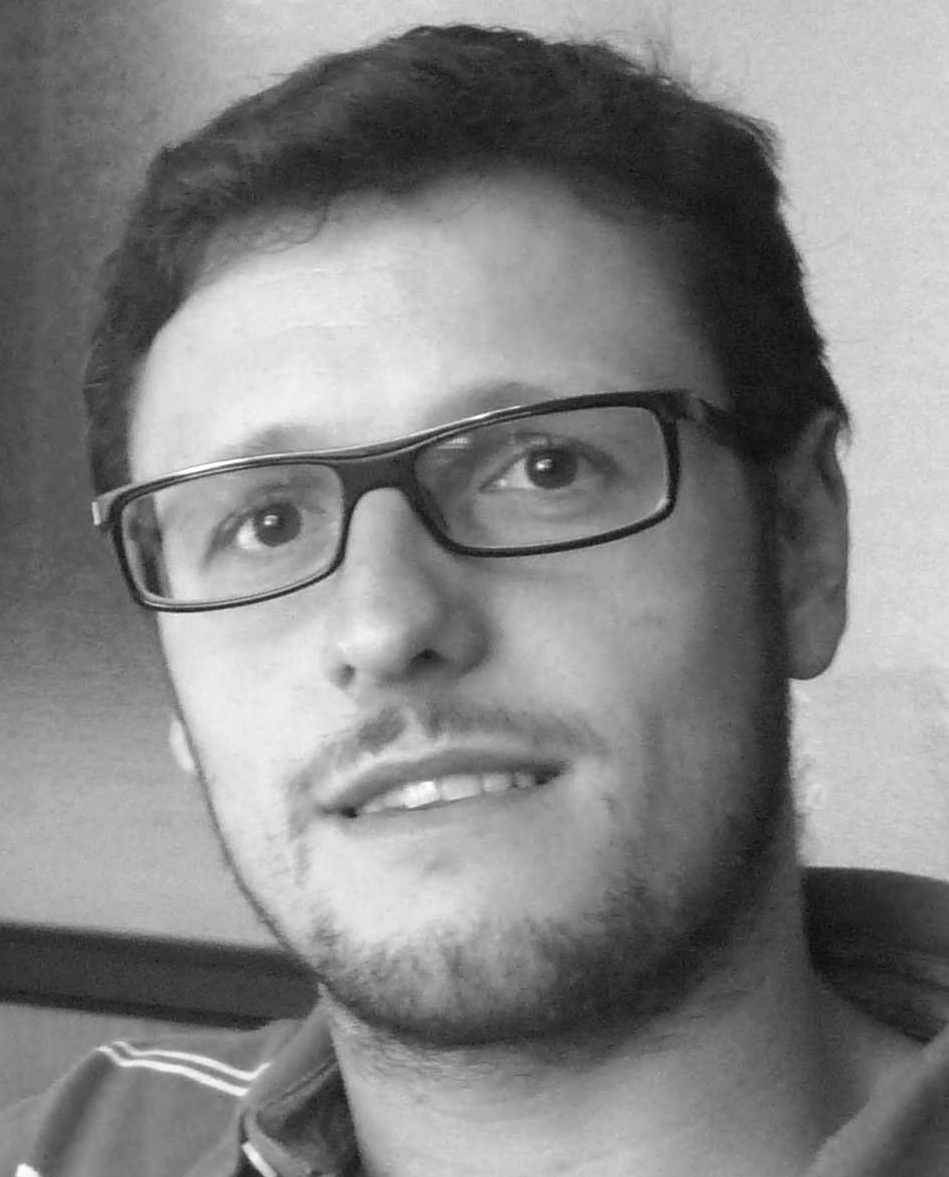
\includegraphics[width=0.7\textwidth]{foto}
		\caption*{GOD BLESS OUR SAVIOUR}
	\end{figure}
	\backmatter
	\printindex
\end{document}